\marginpar{
\vspace{-4in}
\begin{figure}
  \begin{center}
  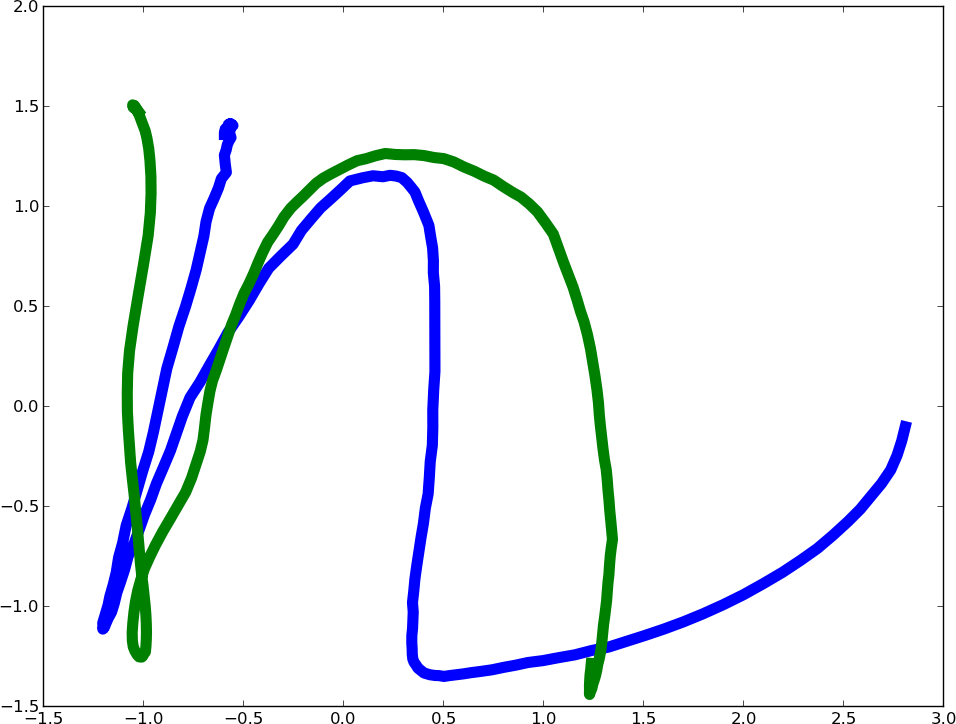
\includegraphics[width=1.5in]{images/new-n-match-cropped.png}
  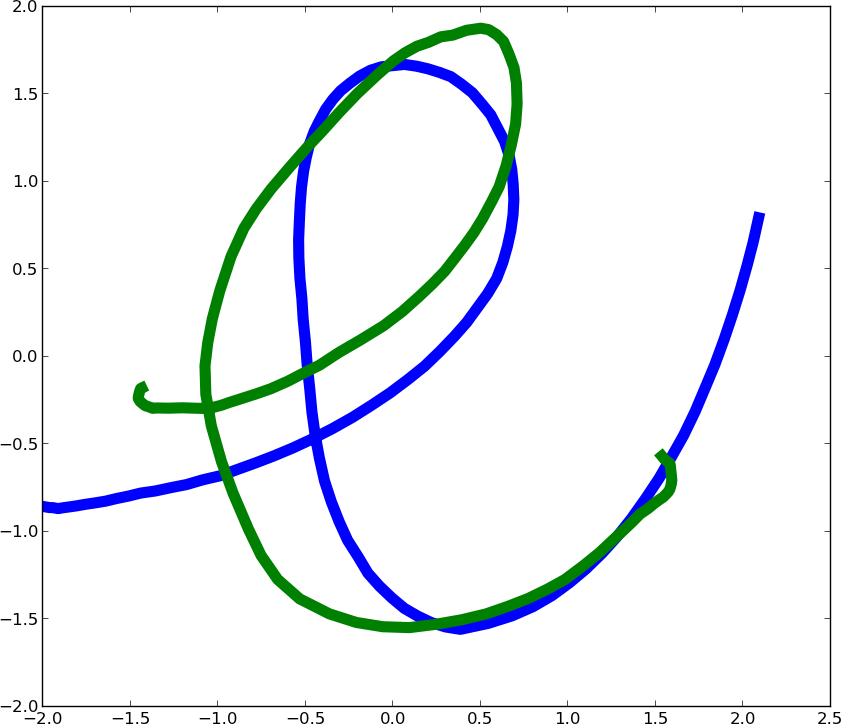
\includegraphics[width=1.5in]{images/new-e-match-cropped.png}
  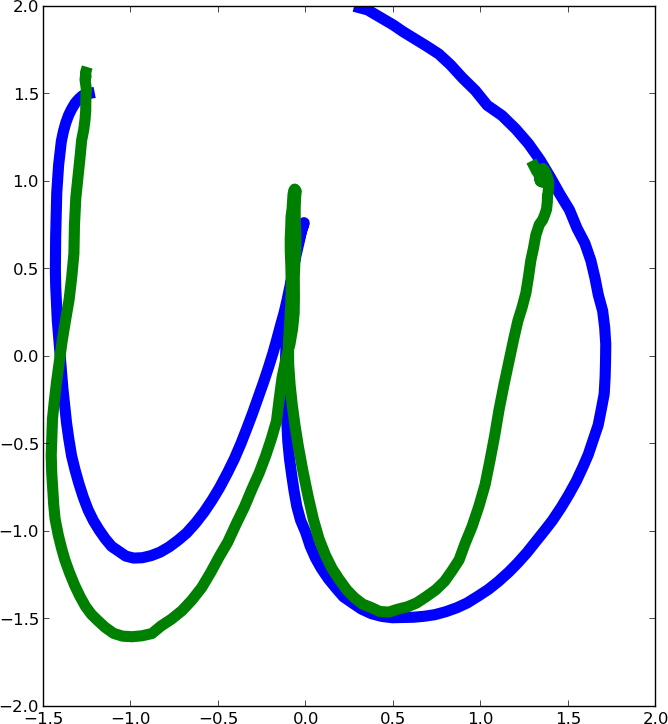
\includegraphics[width=1.5in]{images/new-w-match-cropped.png}
  \caption{The "n", "e", and "w" matches for the "new" time series. Candidates are in green and subsequences from the data are in blue.} \label{fig12}
  \label{fig:teaser}
  \end{center}  
\end{figure}
}

Preliminary tests on the algorithm have been run. Using database sizes of 30 and 168 recordings, with DTW windows of 0, 1, 5, and 10, similarity searches have been run, getting one-nearest-neighbour matches for each candidate in the database.

\begin{table}
\begin{center}
\caption{Times of non-parallelized similarity search with data length 495 (the word "new")}
\begin{tabular}{ cc|c|c| }
\cline{3-4}
& & \multicolumn{2}{ c| }{Database Size} \\ \cline{3-4}
& & 30 & 168 \\ \cline{1-4}
\multicolumn{1}{ |c| }{\multirow{4}{*}{DTW Window} } &
\multicolumn{1}{ |c| }{0} & 1.02s & 6.03s  \\ \cline{2-4} 
\multicolumn{1}{ |c  }{}                        &
\multicolumn{1}{ |c| }{1} & 1.55s & 6.56s  \\ \cline{2-4} 
\multicolumn{1}{ |c  }{}                        &
\multicolumn{1}{ |c| }{5} & 1.77s & 7.51s \\ \cline{2-4} 
\multicolumn{1}{ |c  }{}                        &
\multicolumn{1}{ |c| }{10} & 2.16s & 9.81s \\ \cline{1-4} 
\end{tabular}
\end{center}
\end{table}

An example test time series was the word "new," taken from The Gettysburg Address. In this query, we were looking for the closest database matches to "new" and their locations. The "new" time series is of length 492 and we ran it with a DTW window of 0. It took 1.02 seconds.
\\
\begin{figure}
    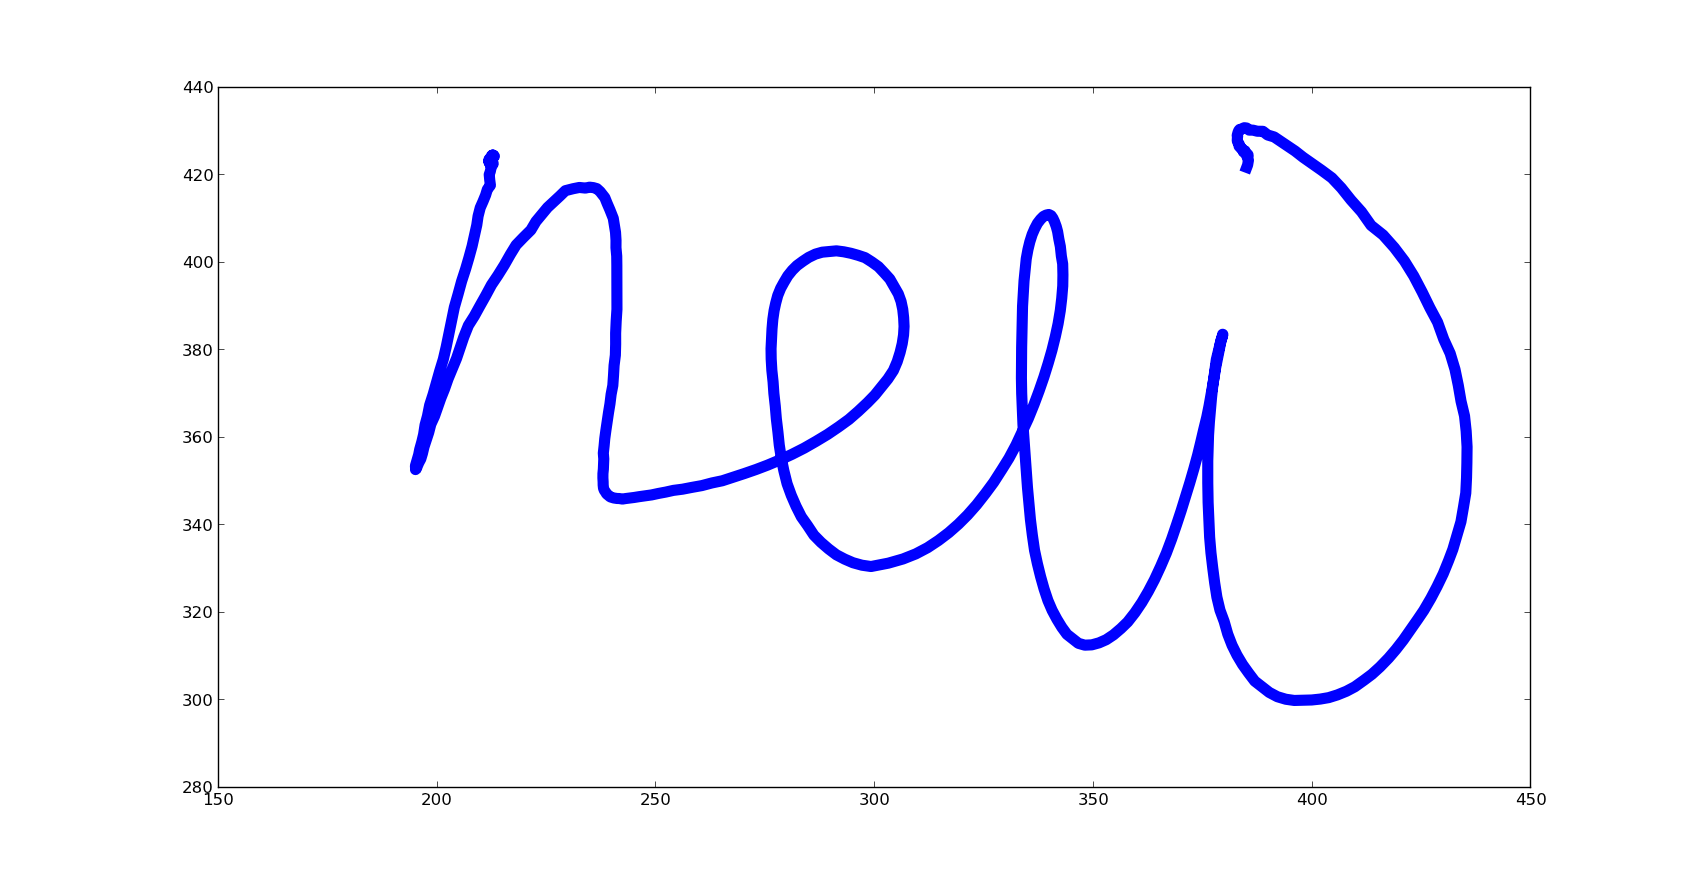
\includegraphics[width=\columnwidth]{images/new-1.png}
    \caption{The "new" time series data}
    \label{fig:teaser}
\end{figure}

The matches for "n", "e", and "w" are pictured in the left margin.
\\
